\begin{figure}[t]
\centering
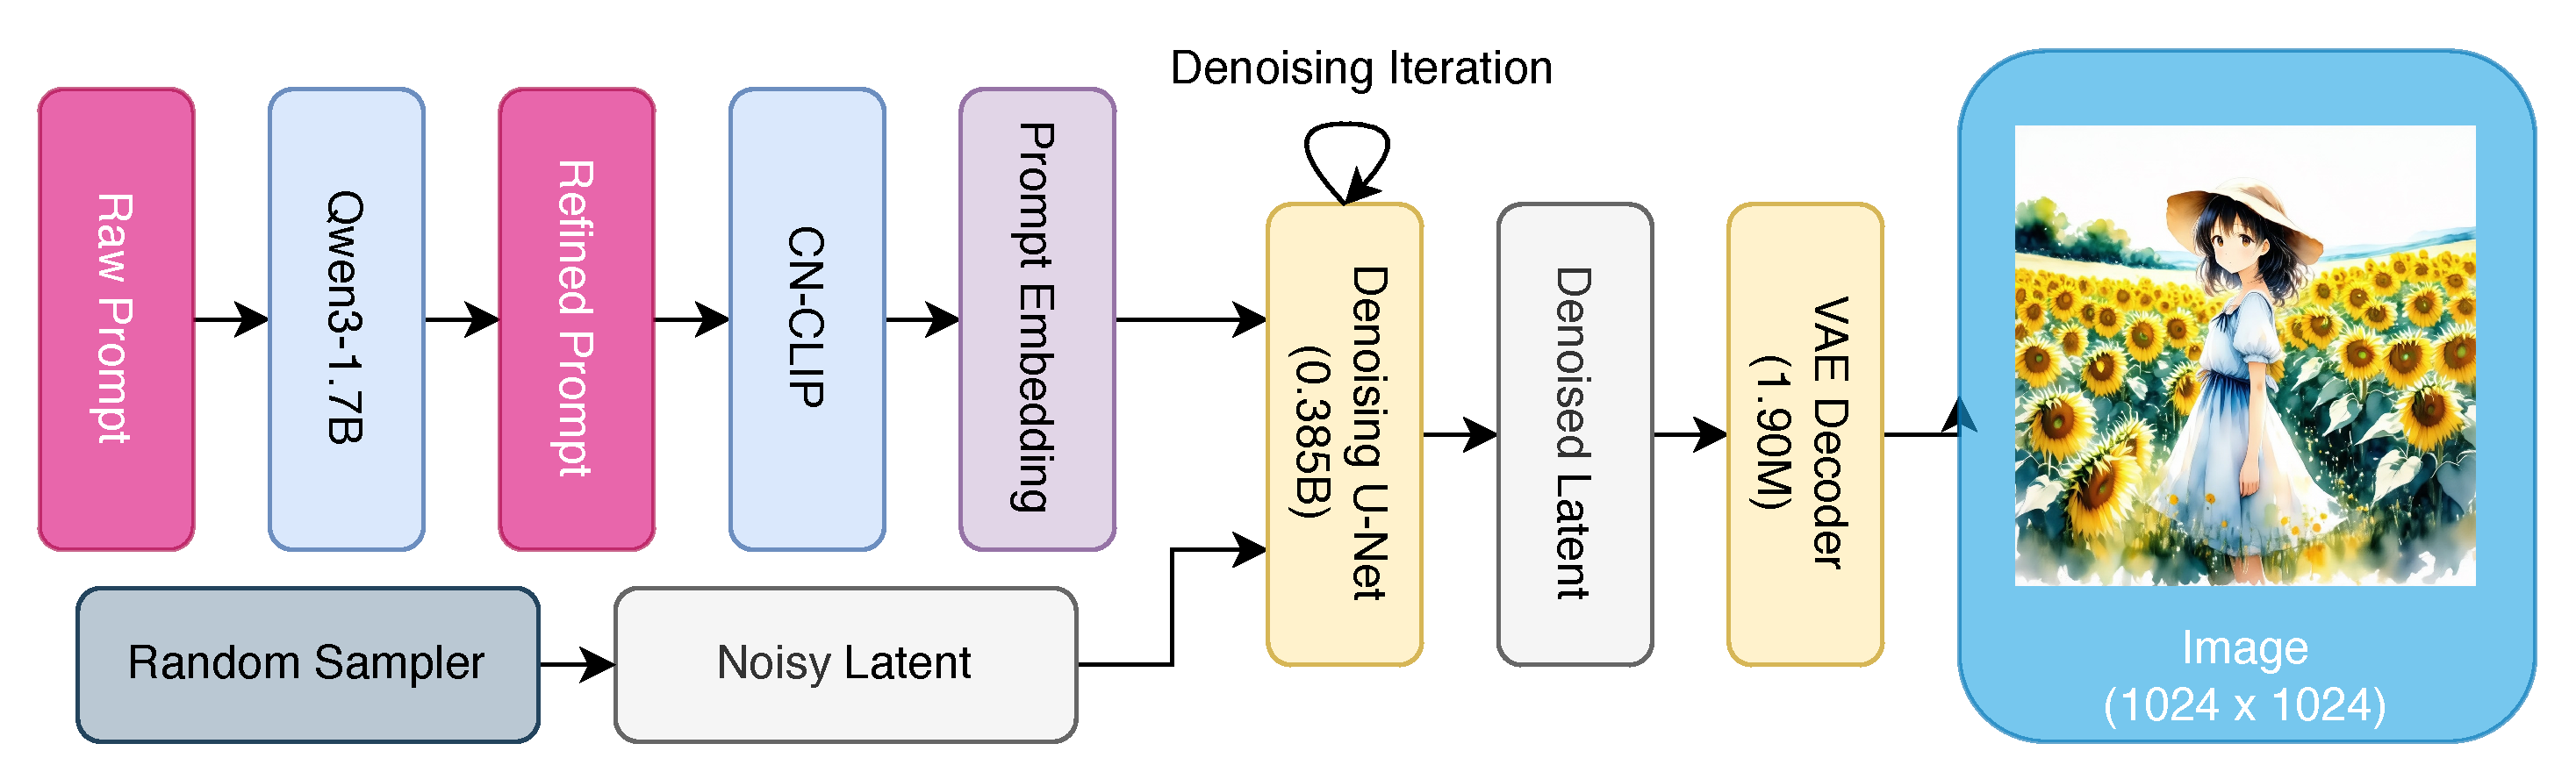
\includegraphics[width=\textwidth]{figures/figures/fig04.pdf}
\caption{\textbf{Overview of the JuZhou 1.0 framework.} A raw poem or user prompt is first refined by Qwen3-1.7B and then encoded by CN-CLIP\protect\footnotemark{} to obtain Chinese semantic conditioning. The conditioning signal is injected into a 0.385B-parameter denoising U-Net for efficient high-resolution generation. The generated latent representation is decoded by an ultra-compact 1.9M-parameter VAE decoder without attention layers. DMD2 distillation further shortens the sampling trajectory from 28 steps to 4 steps, enabling efficient $1024 \times 1024$ image synthesis.}
\label{fig:architecture_overview}
\end{figure}
\footnotetext{The English version adopts CLIP-L and CLIP-G as text encoders, whereas the Chinese version replaces them with Chinese-CLIP ViT-H/14~\cite{chinese-clip}.}

% \begin{table}[t]
%     \centering
%     \caption{Architectural comparison between JuZhou 1.0 and mainstream text-to-image diffusion models. JuZhou 1.0 achieves an 85\% parameter reduction in the denoising network and 98\% in the VAE decoder through systematic architectural simplification.}
%     \label{tab:architecture_comparison}
%     \small
%     \setlength{\tabcolsep}{4.5pt}
%     \begin{tabular}{lcccc}
%         \toprule
%         \textbf{Model} & \textbf{Denoiser + VAE Dec.} & \textbf{Denoiser} & \textbf{VAE Dec.} & \textbf{Mobile} \\
%         \midrule
%         Stable Diffusion v1.5   & $\sim$0.91B & $\sim$0.86B & $\sim$49.49M & {\color{red}\ding{55}} \\
%         Stable Diffusion v2.1   & $\sim$0.92B & $\sim$0.87B & $\sim$49.49M & {\color{red}\ding{55}} \\
%         SDXL 1.0 Base           & $\sim$2.62B & $\sim$2.57B & $\sim$49.49M & {\color{red}\ding{55}} \\
%         Stable Diffusion 3.5 Large & $\sim$8.11B & $\sim$8.06B & $\sim$49.55M & {\color{red}\ding{55}} \\
%         LCM-DreamShaper v7      & $\sim$0.91B & $\sim$0.86B & $\sim$49.49M & {\color{red}\ding{55}} \\
%         SDXL-Lightning 4-Step   & $\sim$2.57B & $\sim$2.57B & - & {\color{red}\ding{55}} \\
%         Sana-600M-1024px        & $\sim$0.59B & $\sim$0.59B & - & {\color{red}\ding{55}} \\
%         \midrule
%         \rowcolor{DeepTeal!10} \textbf{JuZhou 1.0 (Ours)} & $\sim$\textbf{0.387B} & $\sim$\textbf{0.385B} & $\sim$\textbf{1.9M} & {\color{green}\ding{51}} \\
%         \bottomrule
%     \end{tabular}
% \end{table}
% \begin{table}[t]
%     \centering
%     \caption{Architectural comparison between JuZhou 1.0 and mainstream text-to-image diffusion models. JuZhou 1.0 achieves an 85\% parameter reduction in the denoising network and 96\% in the VAE decoder through systematic architectural simplification.}
%     \label{tab:architecture_comparison}
%     \small
%     \setlength{\tabcolsep}{4.5pt}
%     \begin{tabular}{lcccc}
%         \toprule
%         \textbf{Model} & \textbf{Denoiser + VAE Dec.} & \textbf{Denoiser} & \textbf{VAE Dec.} & \textbf{Mobile} \\
%         \midrule
%         Stable Diffusion v1.5      & $\sim$0.91B & $\sim$0.86B & $\sim$49.49M & {\color{red}\ding{55}} \\
%         Stable Diffusion v2.1      & $\sim$0.92B & $\sim$0.87B & $\sim$49.49M & {\color{red}\ding{55}} \\
%         SDXL 1.0 Base              & $\sim$2.62B & $\sim$2.57B & $\sim$49.49M & {\color{red}\ding{55}} \\
%         Stable Diffusion 3.5 Large & $\sim$8.11B & $\sim$8.06B & $\sim$49.55M & {\color{red}\ding{55}} \\
%         LCM-DreamShaper v7         & $\sim$0.91B & $\sim$0.86B & $\sim$49.49M & {\color{red}\ding{55}} \\
%         SDXL-Lightning 4-Step      & $\sim$2.57B & $\sim$2.57B & -             & {\color{red}\ding{55}} \\
%         Sana-600M-1024px           & $\sim$0.59B & $\sim$0.59B & -             & {\color{red}\ding{55}} \\
%         MobileDiffusion            & \textit{$\sim$0.396B} & \textit{$\sim$0.386B} & \textit{$\sim$9.8M}  & {\color{green}\ding{51}} \\
%         SnapGen                    & \textbf{$\sim$0.373B} & \textbf{$\sim$0.372B} & \textbf{$\sim$1.38M} & {\color{green}\ding{51}} \\
%         \midrule
%         \rowcolor{DeepTeal!10} \textbf{JuZhou 1.0 (Ours)}
%         & \underline{$\sim$0.387B}
%         & \underline{$\sim$0.385B}
%         & \underline{$\sim$1.90M}
%         & {\color{green}\ding{51}} \\
%         \bottomrule
%     \end{tabular}
% \end{table}

\begin{table}[t]
    \centering
    \fontsize{7.2pt}{8.2pt}\selectfont
    \setlength{\tabcolsep}{2.0pt}

    % ---------- Left table ----------
    \begin{minipage}[t]{0.64\linewidth}
        \centering
        \caption{Architectural comparison between JuZhou 1.0 and mainstream text-to-image diffusion models.}
        \label{tab:architecture_comparison}

        \renewcommand{\arraystretch}{1.08}
        \begin{tabular*}{\linewidth}{@{\extracolsep{\fill}}lcccc@{}}
            \toprule
            \textbf{Model} & \textbf{Denoiser+VAE} & \textbf{Denoiser} & \textbf{VAE} & \textbf{Mobile} \\
            \midrule
            SD v1.5              & $\sim$0.91B & $\sim$0.86B & $\sim$49.49M & {\color{red}\ding{55}} \\
            SD v2.1              & $\sim$0.92B & $\sim$0.87B & $\sim$49.49M & {\color{red}\ding{55}} \\
            SDXL 1.0 Base        & $\sim$2.62B & $\sim$2.57B & $\sim$49.49M & {\color{red}\ding{55}} \\
            SD 3.5 Large         & $\sim$8.11B & $\sim$8.06B & $\sim$49.55M & {\color{red}\ding{55}} \\
            LCM-DreamShaper v7   & $\sim$0.91B & $\sim$0.86B & $\sim$49.49M & {\color{red}\ding{55}} \\
            SDXL-Lightning 4-Step& $\sim$2.57B & $\sim$2.57B & --           & {\color{red}\ding{55}} \\
            Sana-600M-1024px     & $\sim$0.59B & $\sim$0.59B & --           & {\color{red}\ding{55}} \\
            MobileDiffusion      & \textit{$\sim$0.396B} & \textit{$\sim$0.386B} & \textit{$\sim$9.8M}  & {\color{green}\ding{51}} \\
            SnapGen              & \textbf{$\sim$0.373B} & \textbf{$\sim$0.372B} & \textbf{$\sim$1.38M} & {\color{green}\ding{51}} \\
            \midrule
            \textbf{JuZhou 1.0}
            & \underline{$\sim$0.387B}
            & \underline{$\sim$0.385B}
            & \underline{$\sim$1.90M}
            & {\color{green}\ding{51}} \\
            \bottomrule
        \end{tabular*}
    \end{minipage}
    \hspace{0.025\linewidth}
    % ---------- Right table ----------
    \begin{minipage}[t]{0.30\linewidth}
        \vspace{0pt}
        \centering
        \caption{K100 training cluster specifications.}
        \label{tab:k100_specs}
    
        \renewcommand{\arraystretch}{1.09}
        \begin{tabular*}{\linewidth}{@{\extracolsep{\fill}}ll@{}}
            \toprule
            \textbf{Spec.} & \textbf{Value} \\
            \midrule
            Accelerator & Hygon DCU K100 \\
            FP16/BF16 Perf. & 196 TFLOPS \\
            HBM3 & 64 GB \\
            Mem. Bandwidth & 896 GB/s \\
            Host Interface & PCIe 5.0 x16 \\
            Ecosystem & ROCm \\
            \midrule
            Nodes & 56 \\
            Accel./Node & 4 \\
            Total Accel. & 224 \\
            Interconnect & InfiniBand RDMA \\
            \bottomrule
        \end{tabular*}
    \end{minipage}

    \renewcommand{\arraystretch}{1.0}
\end{table}

\section{Ultra-Lightweight Architecture Design}

To enable high-resolution text-to-image generation on resource-constrained edge devices, JuZhou 1.0 adopts an ultra-lightweight architecture centered on a compact denoising U-Net and a highly compressed VAE decoder. As illustrated in Fig.~\ref{fig:architecture_overview}, a raw poem or user prompt is first refined by the lightweight prompt refiner and then encoded by the Chinese text encoder to obtain semantic conditioning. 
% The conditioning signal is injected into a 0.4B-parameter denoising U-Net for latent-space generation, and the resulting latent representation is decoded by a 1.9M-parameter attention-free VAE decoder. 
The conditioning signal is injected into a 0.385B-parameter denoising U-Net for latent-space generation, and the resulting latent representation is decoded by a 1.90M-parameter attention-free VAE decoder. Together, the denoiser and decoder contain approximately 0.387B parameters; the rounded 0.4B figure refers only to this image-generation backbone.
DMD2 distillation further reduces sampling from 28 to 4 steps, enabling efficient $1024 \times 1024$ synthesis.
% Tab.~\ref{tab:architecture_comparison} compares the parameter scale of JuZhou 1.0 with mainstream text-to-image diffusion models. 
% The following subsections detail the lightweight denoising network and the compact VAE decoder, respectively.
Tab.~\ref{tab:architecture_comparison} compares JuZhou 1.0 with mainstream text-to-image diffusion models in parameter scale. We then introduce the lightweight denoising network and compact VAE decoder.

\subsection{Denoising Network}
\begin{figure}[t]
\centering
\captionsetup{skip=6pt}
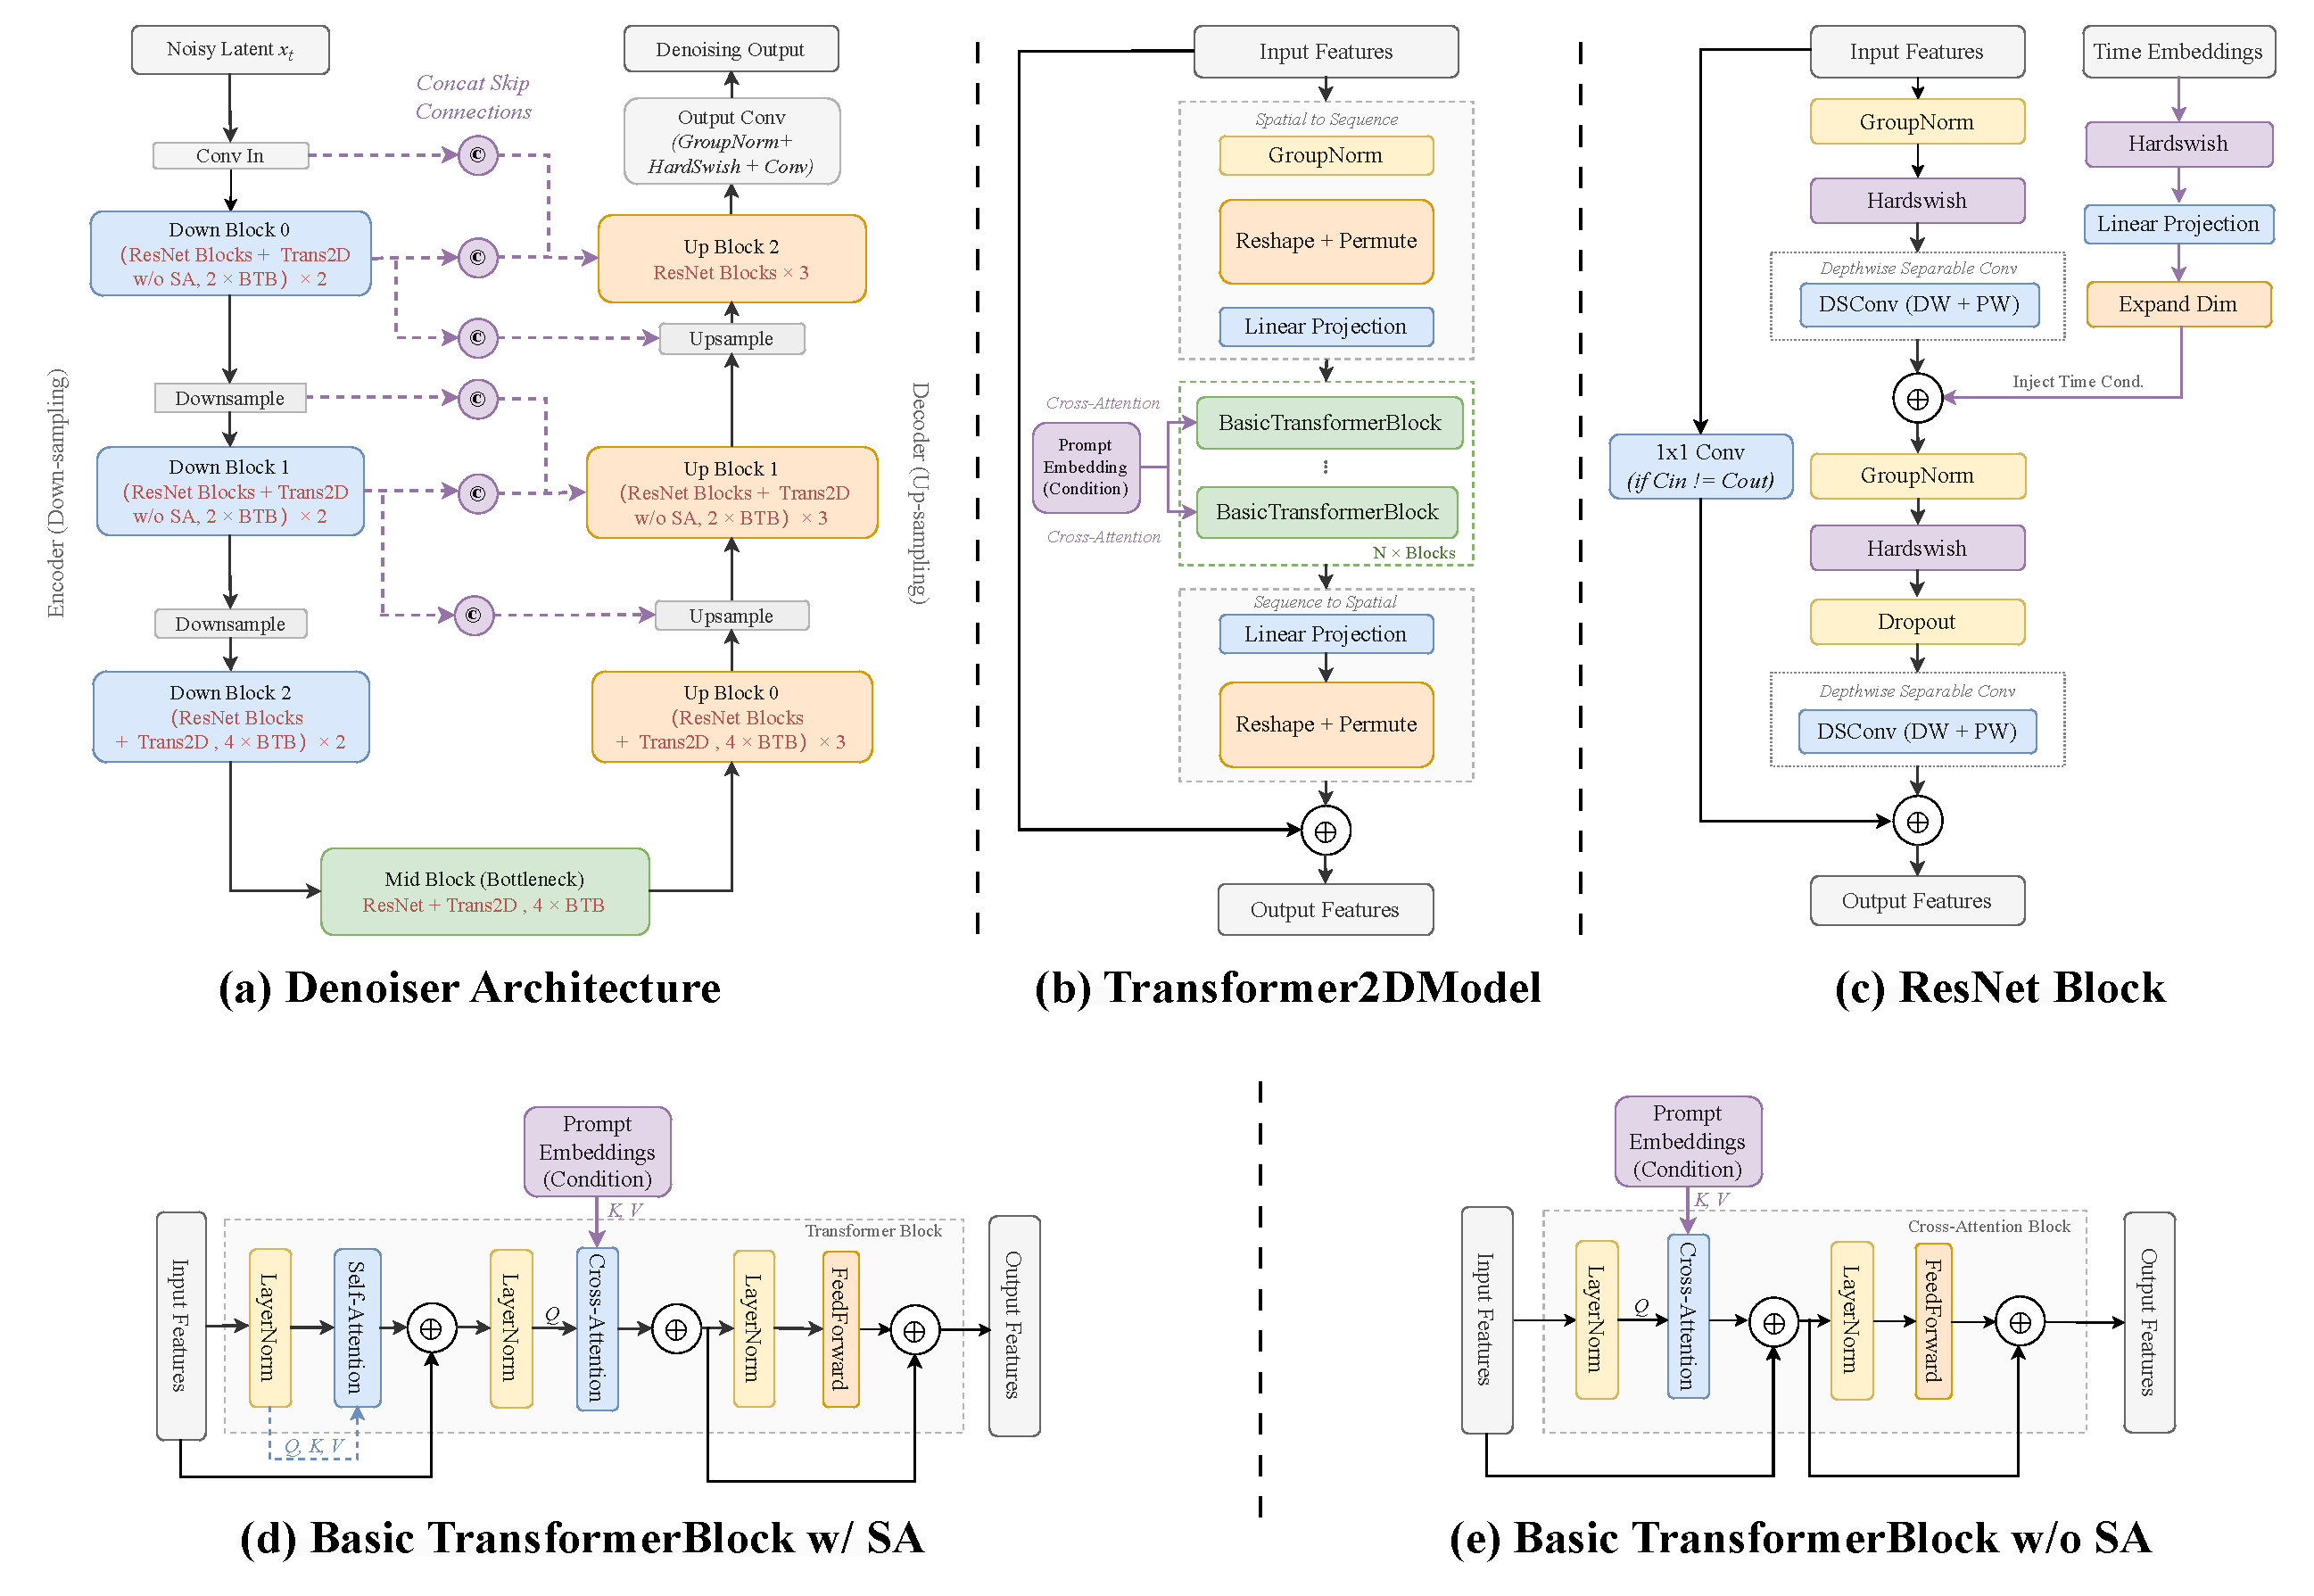
\includegraphics[ width=\textwidth, trim=0 20pt 0 0, clip ]{figures/figures/008.pdf}
\caption{Overview of the lightweight denoising network. (a) Denoiser architecture. (b) Transformer2DModel. (c) ResNet Block. (d) BasicTransformerBlock w/ SA. (e) BasicTransformerBlock w/o SA. BTB denotes BasicTransformerBlock, and SA denotes self-attention. }
\label{fig:denoising_overview}
\end{figure}

\begin{figure}[t]
\centering
\captionsetup{skip=6pt}
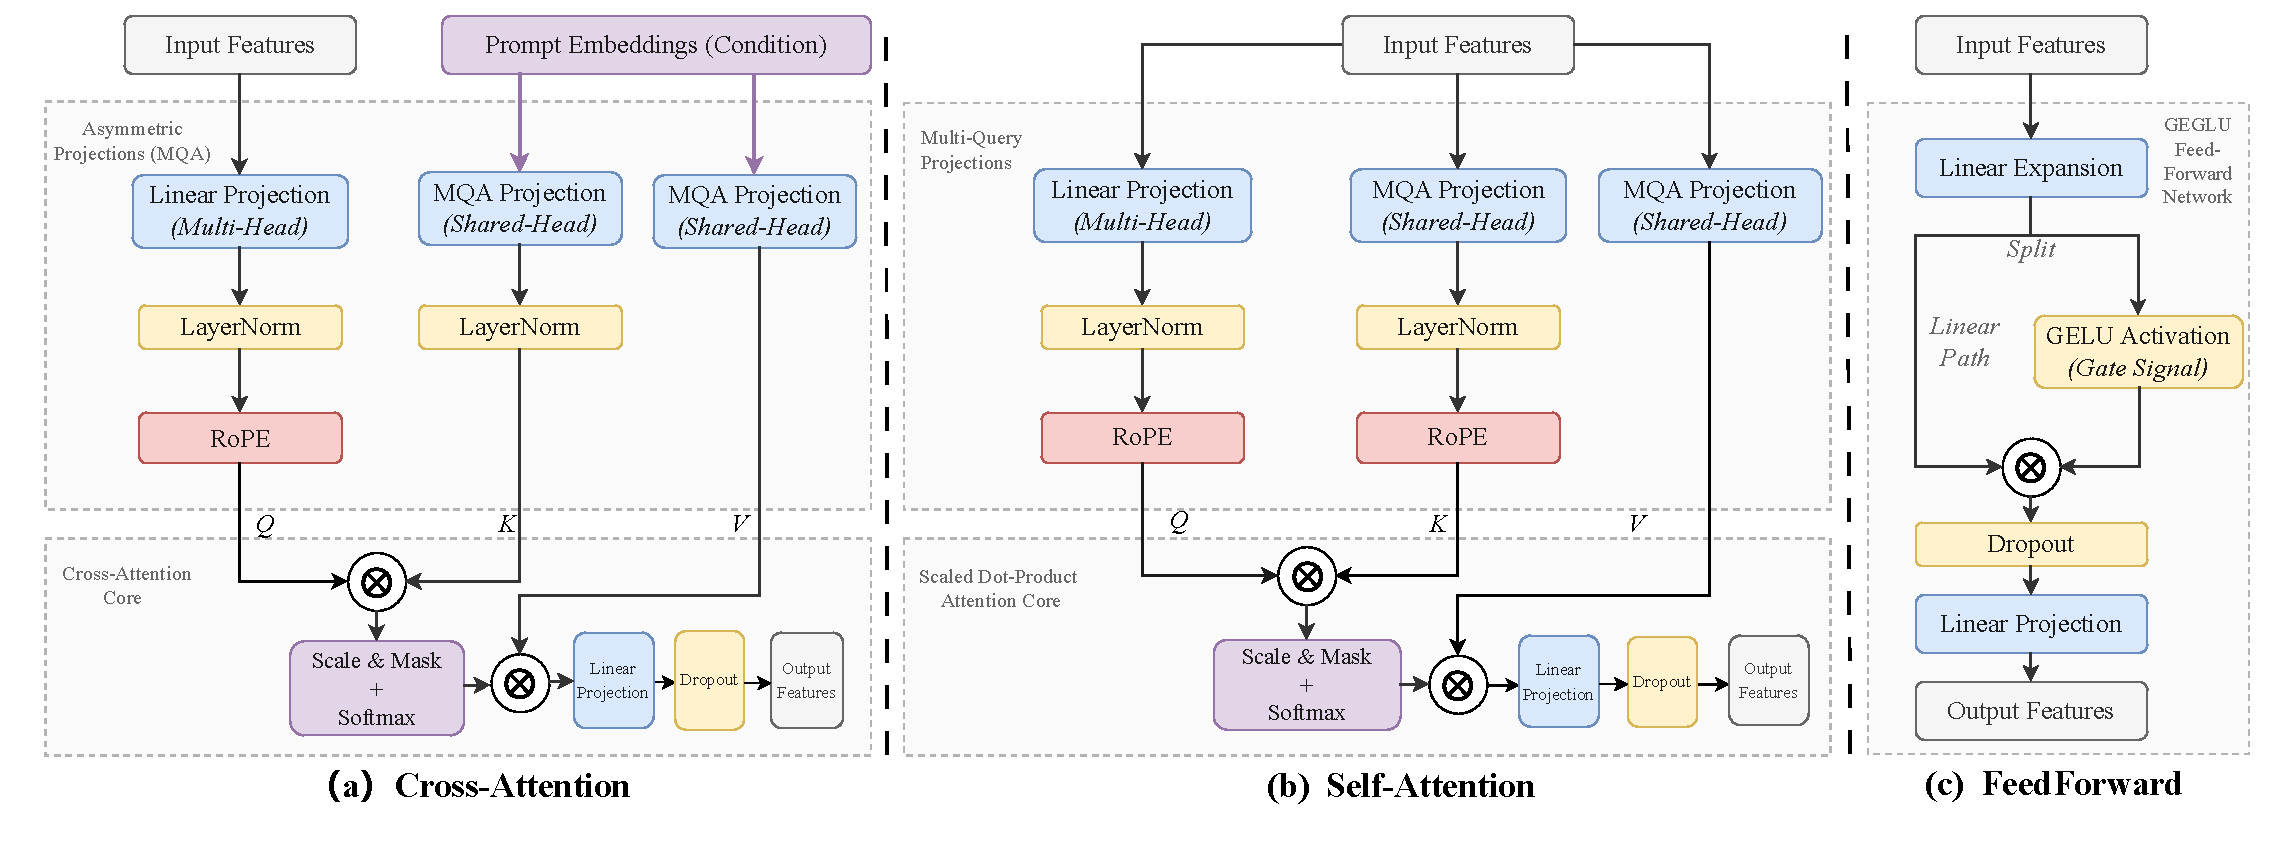
\includegraphics[ width=\textwidth, trim=0 20pt 0 0, clip ]{figures/figures/009.pdf}
\caption{Detailed modules in the denoising network. (a) Cross-attention. (b) Self-attention. (c) GEGLU-based feed-forward network. }
\label{fig:denoising_Detailed_modules}
\end{figure}

As illustrated in Fig.~\ref{fig:denoising_overview}, the denoising network follows an encoder--bottleneck--decoder U-Net structure while substantially reducing the parameter count and computational cost. Given an input latent representation ($x_t$), the model first projects it into the backbone feature space using a ($3 \times 3$) convolutional input layer. The encoder consists of three down blocks, each combining ResNet blocks with Transformer2D modules to capture both local spatial patterns and text-conditioned semantics. After the encoder, the middle block further integrates ResNet blocks with Transformer2D modules to refine the bottleneck representation through global semantic interactions. The decoder contains three resolution-aware up blocks, where the first two up blocks also integrate ResNet blocks with Transformer2D modules, while the final up block is composed only of ResNet blocks. The decoder progressively recovers spatial resolution and produces the final denoising prediction through an output projection head composed of GroupNorm, Hardswish, and a ($3 \times 3$) convolution.

The detailed attention and feed-forward modules used in the denoising network are shown in Fig.~\ref{fig:denoising_Detailed_modules}. 
% To improve efficiency, the network reduces redundant high-resolution computation and selectively allocates attention operations according to the resolution and semantic modeling requirements of each stage. 
To improve efficiency, the network reduces high-resolution redundancy and selectively applies attention based on stage-specific resolution and semantic needs.
Specifically, the Transformer2D modules in the first two down blocks and the first two up blocks remove self-attention and retain only cross-attention, allowing text-conditioned feature modulation with lower computational cost. In contrast, the remaining Transformer-equipped stages, including the third down block and the middle block, employ both self-attention and cross-attention to enhance global spatial reasoning and text-image interaction. Within each ResNet block, GroupNorm and Hardswish are used to stabilize training and provide hardware-friendly nonlinear transformation. 
% In the Transformer2D modules, the attention inputs are normalized by LayerNorm before attention computation, enabling stable feature interaction under a compact model budget.
% In Transformer2D, LayerNorm stabilizes attention-based feature interaction under a compact model budget.
In Transformer2D modules, LayerNorm is applied before attention and feed-forward operations to stabilize feature interactions under the compact model capacity.

The skip connections are redesigned to preserve multi-scale spatial details while reducing redundant feature fusion near the bottleneck. Specifically, the shallow features from the input convolution are directly connected to the highest-resolution decoder stage, while selected features from Down Block 0 and Down Block 1 are fused into the intermediate upsampling and decoder stages. In contrast, the skip connection from Down Block 2 to Up Block 0 is removed to avoid unnecessary bottleneck-level feature transfer. These lightweight multi-scale skip pathways help the decoder recover local structures and semantic details without substantially increasing model capacity.

\subsection{VAE Decoder}
% \begin{figure}[t]
% \centering
% 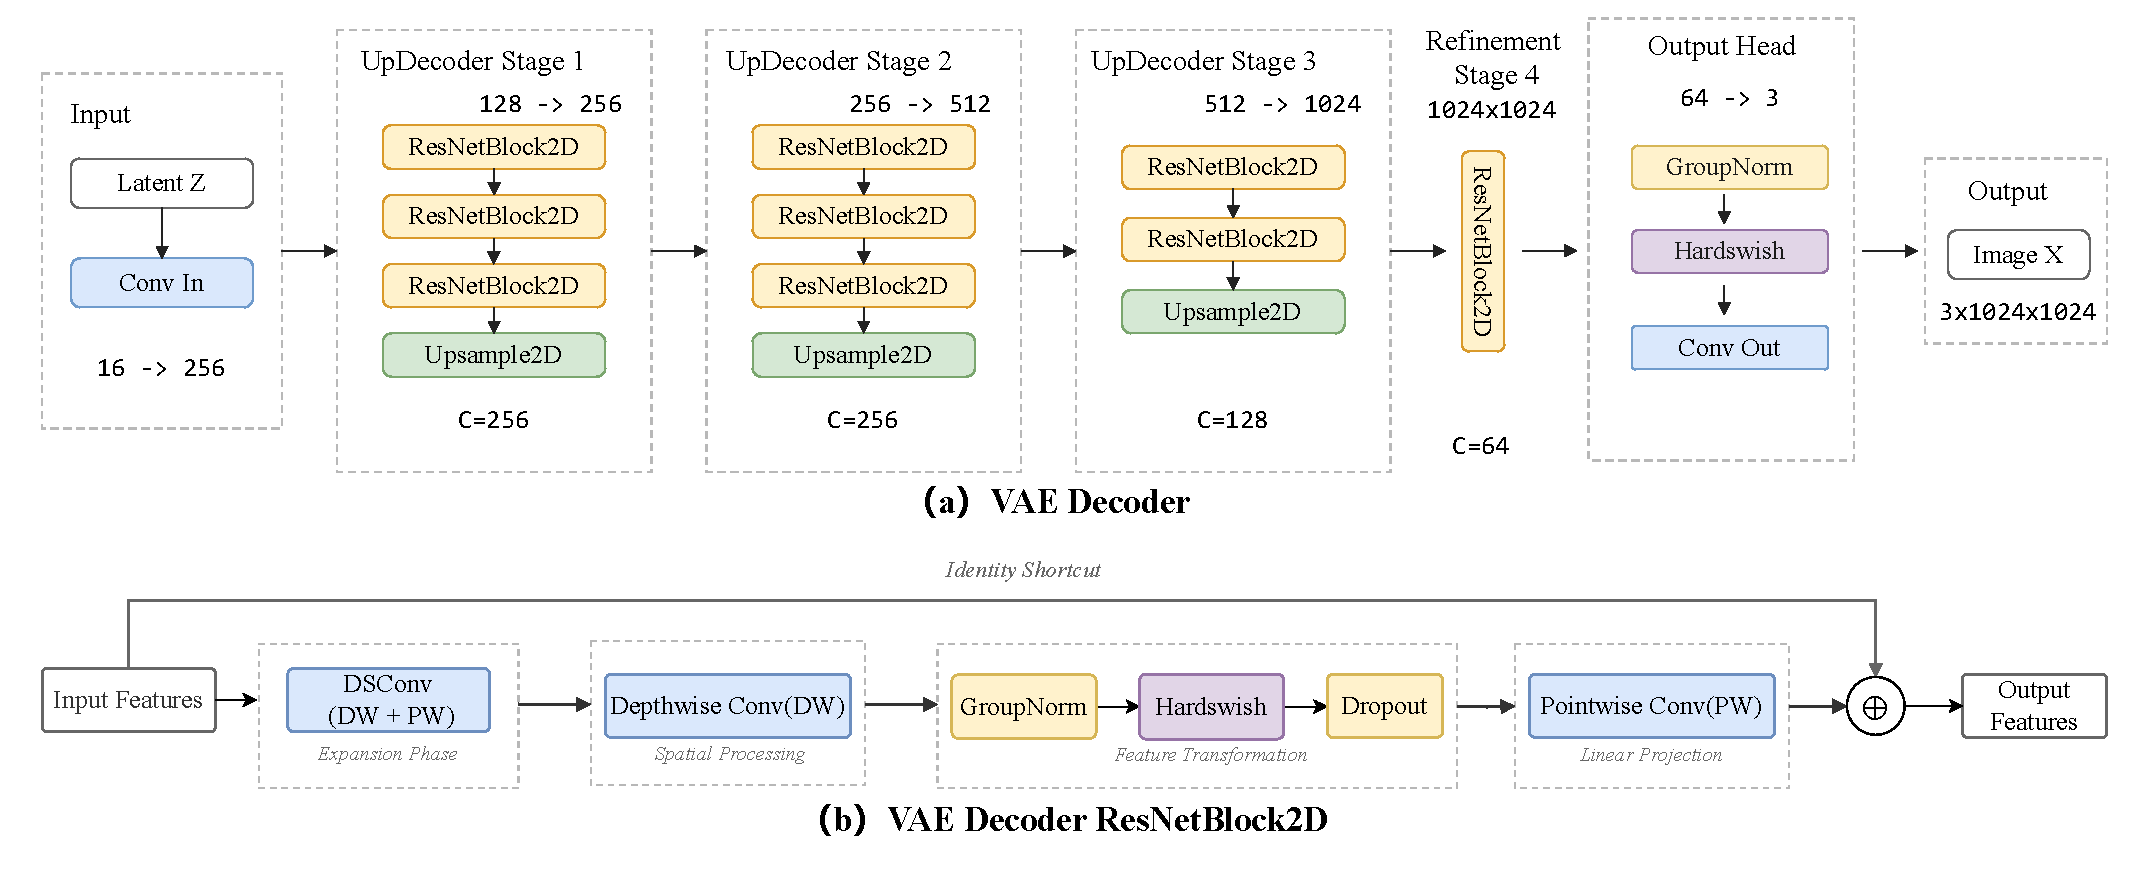
\includegraphics[width=\textwidth]{figures/figures/010.pdf}
% \caption{ Overview of the compact VAE decoder. (a) VAE decoder architecture. (b) VAE Decoder ResNetBlock2D. }
% \label{fig:VAE_decoder_overview}
% \end{figure}
\begin{figure}[t]
\centering
\captionsetup{skip=4pt}
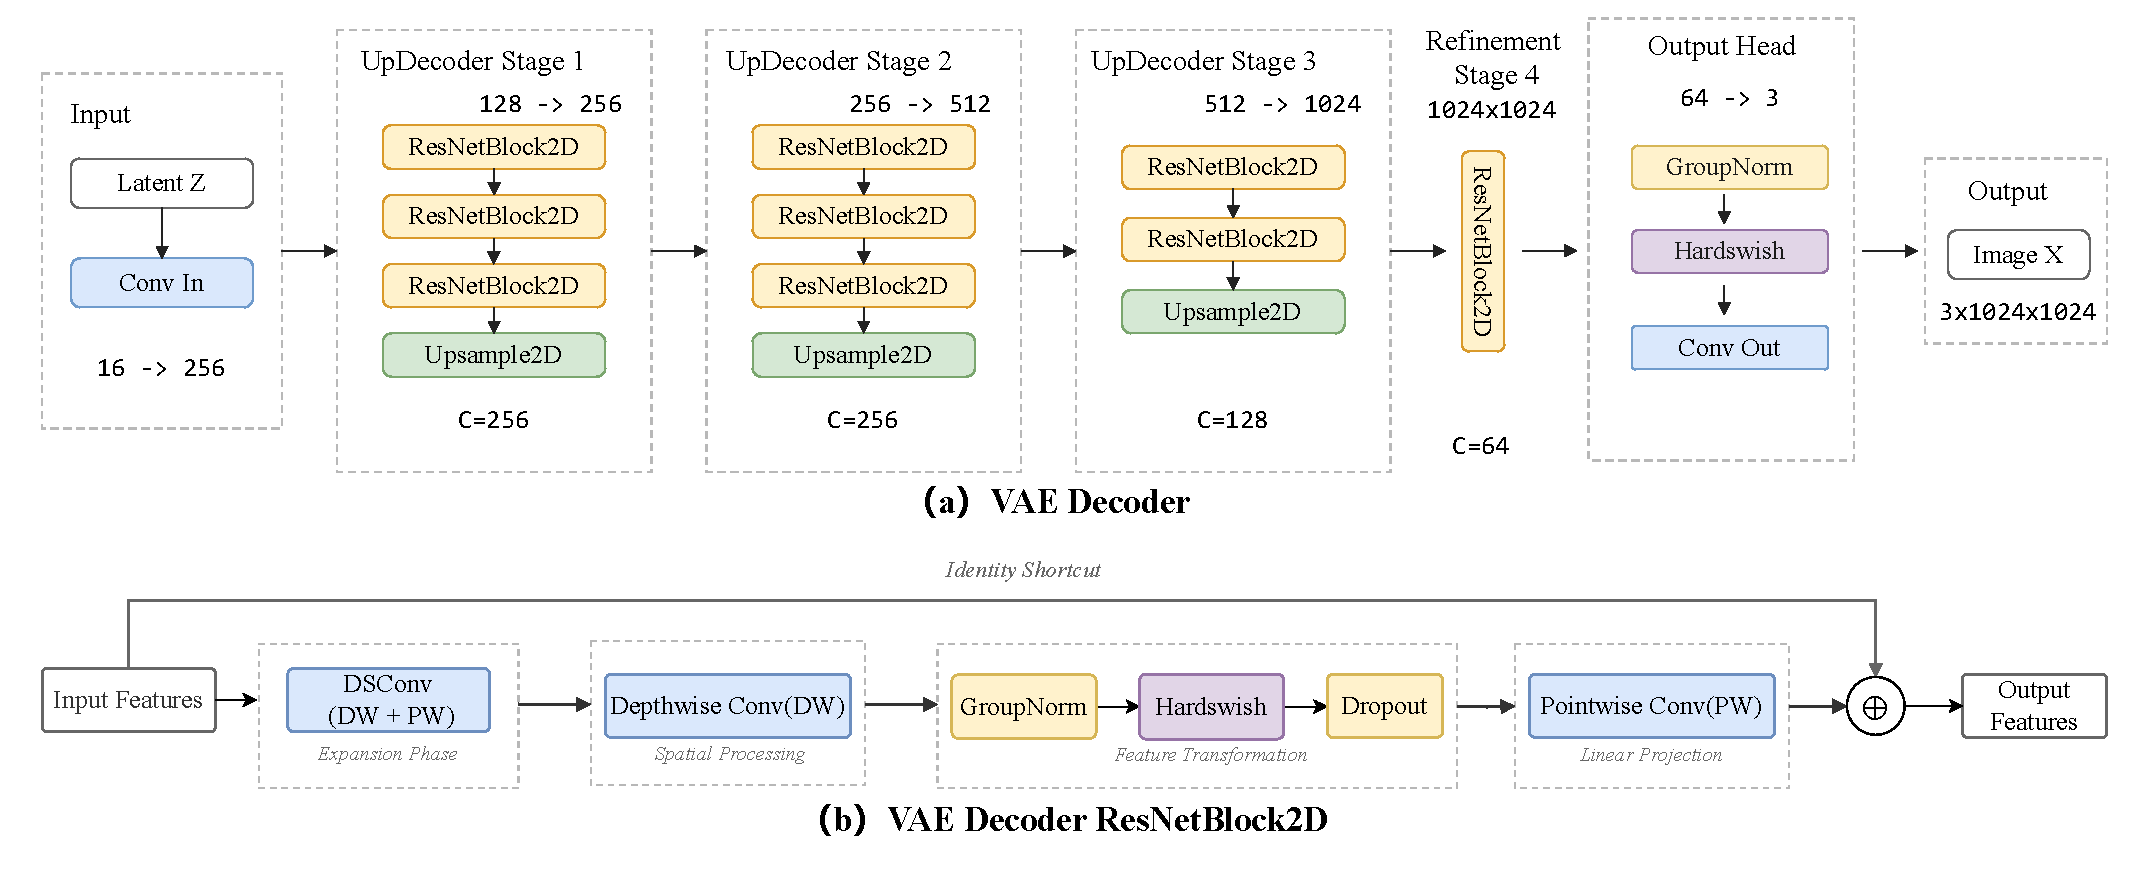
\includegraphics[
    width=\textwidth,
    trim=0 20pt 0 0,
    clip
]{figures/figures/010.pdf}
\caption{Overview of the compact VAE decoder. (a) VAE decoder architecture. (b) VAE decoder ResNetBlock2D.}
\label{fig:VAE_decoder_overview}
\end{figure}

% As shown in Fig.~\ref{fig:VAE_decoder_overview}, the image decoding stage is a major memory bottleneck for on-device generative models, especially when producing high-resolution images. To reduce both parameter storage and peak activation memory, we redesign the VAE decoder as a compact attention-free architecture. The decoder first projects the 16-channel latent representation into a 256-channel feature map through a convolutional input layer. It is then organized into several decoder blocks with channel widths of 256, 256, 128, and 64, progressively recovering image details while keeping the feature dimension strictly controlled.
As shown in Fig.~\ref{fig:VAE_decoder_overview}, image decoding is a major memory bottleneck for on-device high-resolution generation. We therefore redesign the VAE decoder as a compact attention-free architecture. It projects the 16-channel latent into 256 channels and progressively decodes features with channel widths of 256, 256, 128, and 64, reducing parameter storage and peak activation memory.

% Each decoder block contains multiple lightweight ResNet blocks. Instead of using standard dense convolutions throughout the block, we adopt a depthwise--pointwise convolutional design to reduce convolutional redundancy. Specifically, each block sequentially applies depthwise convolution, pointwise convolution, another depthwise convolution, GroupNorm, Hardswish, Dropout, and a final pointwise convolution. This design preserves local feature transformation capacity while substantially reducing the number of parameters and memory access cost.
% Each decoder block contains multiple lightweight ResNet blocks. Instead of using standard dense convolutions throughout the block, we adopt a depthwise--pointwise convolutional design to reduce convolutional redundancy. Specifically, each block sequentially applies depthwise convolution, pointwise convolution, another depthwise convolution, GroupNorm, Hardswish, Dropout, and a final pointwise convolution. This factorized convolution structure separates spatial filtering from channel mixing, making the decoder more efficient under mobile memory and bandwidth constraints. It also keeps the decoding path attention-free, which helps reduce peak activation memory during high-resolution image reconstruction. This design preserves local feature transformation capacity while substantially reducing the number of parameters and memory access cost.
Each decoder block contains multiple lightweight ResNet blocks. Instead of using standard dense convolutions throughout the block, we adopt a depthwise--pointwise convolutional design to reduce convolutional redundancy. Specifically, each block sequentially applies depthwise convolution, pointwise convolution, another depthwise convolution, GroupNorm, Hardswish, Dropout, and a final pointwise convolution. This factorized structure separates spatial filtering from channel mixing, making the decoder more efficient under mobile memory and bandwidth constraints. The attention-free decoding path further helps reduce peak activation memory during high-resolution image reconstruction, while preserving local feature transformation capacity.

The output head further refines the final 64-channel feature map with an additional lightweight ResNet block, followed by GroupNorm, Hardswish, and a final convolution that maps the feature representation to a 3-channel RGB image. By removing attention layers, narrowing channel widths, and simplifying residual block configurations, the proposed decoder reduces the VAE decoder to approximately 1.9M parameters, making it suitable for memory-constrained mobile deployment.
